%LTeX: language=pt-br
% !TeX root = Apostila_IM381.tex

\cleardoublepage
\section{Revisão modelo de viga}

    Nesta seção, será apresentada uma revisão do modelo de barra, sua equação diferencial, com alguns exemplos e exercícios.

    \subsection{Hipóteses}

        As principais hipóteses do modelo de barra são:

        \begin{itemize}
            \item Estrutura esbelta - comprimento muito maior que sua largura ou espessura;
            \item Material linear elástico isotrópico;
            \item Pequenas deformações e pequenos deslocamentos;
            \item Submetido apenas a forças transversais ou momentos fletores;
            \item Deformações locais desprezíveis (princípio de Saint-Venant).
            \item Seção plana permanece plana após a deformação
        \end{itemize}

    \subsection{Dedução da equação diferencial}

        Considere a viga com uma seção transversal variável, sujeita a forças $q(x)$ (Figura \ref{fig:viga}). Um elemento infinitesimal (Figura \ref{fig:infinitesimal_viga}) dessa viga também deve estar em equilíbrio.

        \begin{figure}[h!]
            \centering
            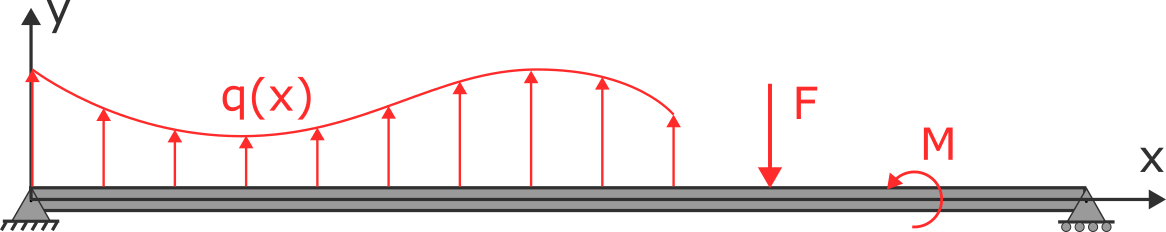
\includegraphics[scale=1]{Figures/5-Viga/Cargas.png}
            \caption{Viga sujeita a esforços externos}
            \label{fig:viga}
        \end{figure}

        \begin{figure}[h!]
            \centering
            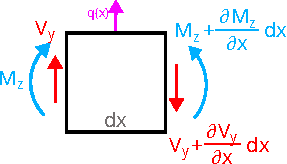
\includegraphics[scale=1.5]{Figures/5-Viga/Infinitesimal.pdf}
            \caption{Elemento infinitesimal de uma viga}
            \label{fig:infinitesimal_viga}
        \end{figure}

        \begin{equation*}
            \sum F_y = 0
        \end{equation*}

        \begin{equation*}
            q(x)dx + V_y - \left(V_y + \frac{dV_y}{dx}dx\right) = 0
        \end{equation*}

        \begin{equation}
            \frac{dV_y}{dx} = q(x)
            \label{eq:viga_dv}
        \end{equation}

        \begin{equation*}
            \sum M_z = 0
        \end{equation*}

        \begin{equation*}
            -V_y\frac{dx}{2} - \left(V_y + \frac{dV_y}{dx}dx\right)\frac{dx}{2} - M_z + \left(M_z + \frac{dM_z}{dx}dx\right) = 0
        \end{equation*}

        \begin{equation*}
            \frac{dM_z}{dx} = V_y + q(x)\frac{dx}{2}
        \end{equation*}

        \begin{equation}
            \frac{dM_z}{dx} = V_y
            \label{eq:viga_dm}
        \end{equation}

        \noindent no qual $M_z(x)$ é chamado momento fletor e $V_y(x)$ é o esforço cortante. Estes são os esforços internos que surgem na estrutura.

        As Eq. \eqref{eq:viga_dv} e Eq. \eqref{eq:viga_dm} representam o equilíbrio do sistema. Podemos juntá-la em:

        \begin{equation}
            \frac{d^2M_z}{dx^2} = q(x)
            \label{eq:viga_equilibrio}
        \end{equation}

        Para a cinemática da viga, consideremos a viga da Figura \ref{fig:deslocamento_viga}, com uma deflexão $v(x)$ e ângulo $\theta(x)$. O modelo mais simples de viga se chama modelo de Euler-Bernoulli. Neste modelo, a deformação devido ao cisalhamento da viga é desprezado. Por exemplo, se pegarmos um livro e dobrarmos, vemos que as folhas dele vão se atritar umas nas outras. No modelo de Euler-Bernoulli, consideramos que as folhas estão todas coladas entre si.

        \begin{figure}[h!]
            \centering
            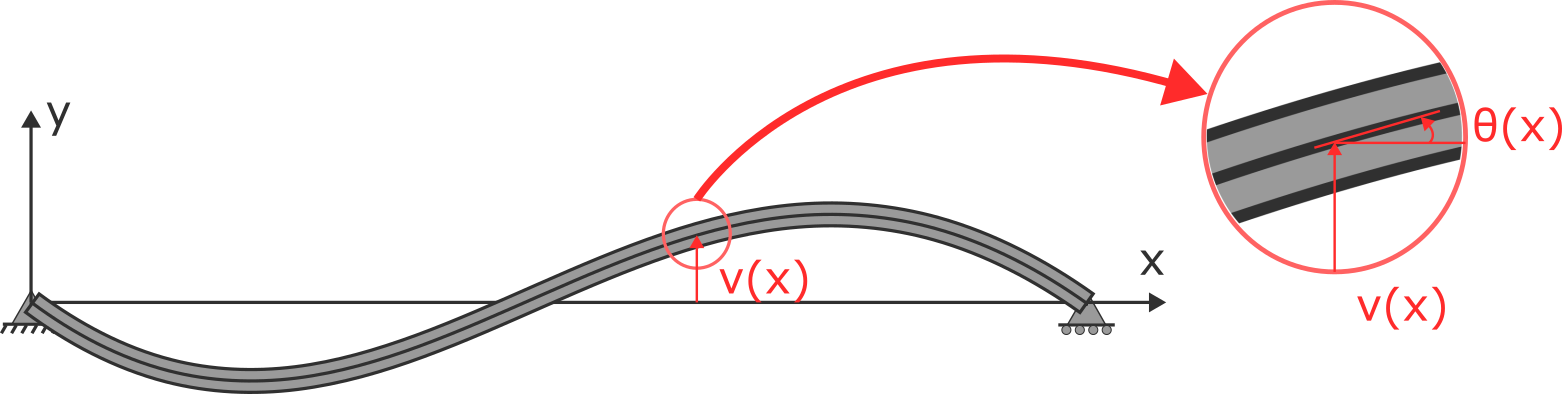
\includegraphics[scale=0.8]{Figures/5-Viga/Deslocado.png}
            \caption{Viga deslocada devido a esforços externos}
            \label{fig:deslocamento_viga}
        \end{figure}

        Considere o elemento infinitesimal não deformado e o deformado (Figura \ref{fig:viga_deform_infinitesimal}). Uma das hipóteses deste modelo, que se verifica na prática, é que suas superfícies planas permanecerão planas, isto é, os lados desse elemento permanecerão retos. O elemento se deformará, formando um arco de disco. Haverá uma linha transversal ao longo do elemento na qual o comprimento deste elemento não altera. Esta linha se chama linha neutra. O raio da circunferência descrita pela linha neutra neste elemento infinitesimal é o raio de curvatura $\rho(x)$.

        \begin{figure}[h!]
            \centering
            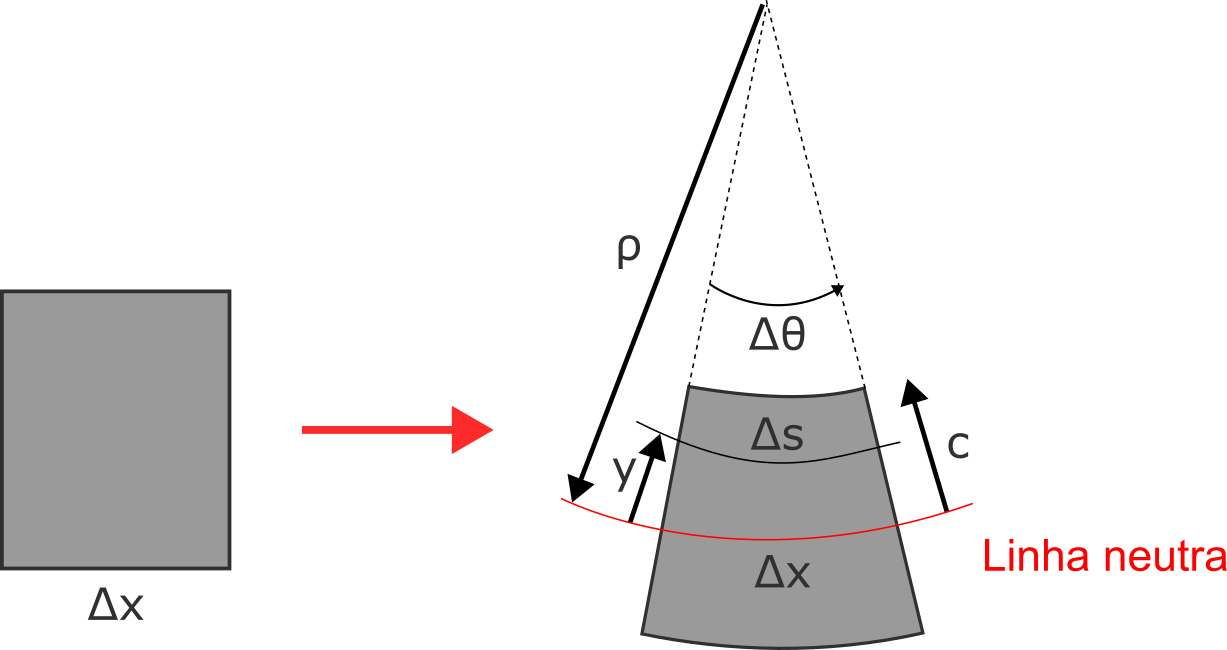
\includegraphics[scale=0.8]{Figures/5-Viga/Cinematica.png}
            \caption{Deformação de um elemento infinitesimal de viga}
            \label{fig:viga_deform_infinitesimal}
        \end{figure}

        A deformação normal ao longo desse elemento é calculada pela variação dos comprimentos desse elemento:

        \begin{equation*}
            \varepsilon_{xx}(x,y) = \lim_{\Delta x \rightarrow 0} \frac{\Delta s - \Delta x}{\Delta x}
        \end{equation*}

        \begin{equation}
            \varepsilon_{xx}(x,y) = -\frac{y}{\rho(x)}
        \end{equation}

        Portanto, a deformação segue um perfil linear, como na Figura \ref{fig:viga_deformacao}. Consequentemente, pela lei de Hooke ($\sigma_{xx} = E \varepsilon_{xx}$), temos que a tensão também será linear (Figura \ref{fig:viga_tensao}):

        \begin{figure}[h!]
            \begin{subfigure}{0.49\textwidth}
                \centering
                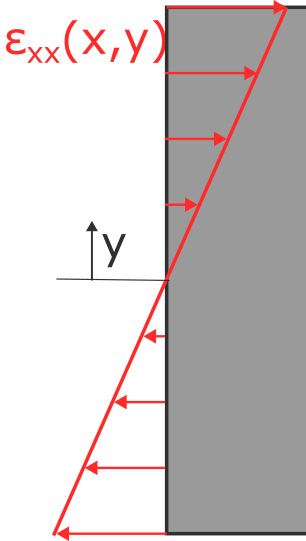
\includegraphics[scale=0.8]{Figures/5-Viga/Deformacao.png}
                \caption{}
                \label{fig:viga_deformacao}
            \end{subfigure}
            ~
            \begin{subfigure}{0.49\textwidth}
                \centering
                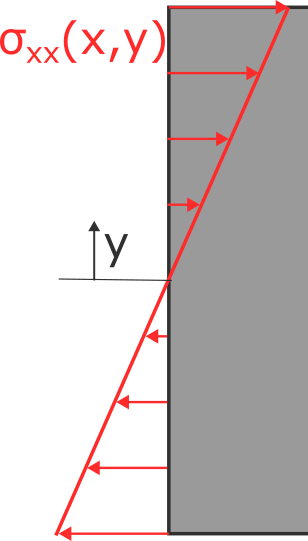
\includegraphics[scale=0.8]{Figures/5-Viga/Tensao.png}
                \caption{}
                \label{fig:viga_tensao}
            \end{subfigure}
            \caption{Tensão e deformação de viga ao longo da seção transversal. (a) Deformação, (b) tensão.}
        \end{figure}


        \begin{equation}
            \sigma_{xx}(x,y) = -\frac{Ey}{\rho(x)}
        \end{equation}

        Considere agora a seção da Figura \ref{fig:equilibrio_secao_viga}. A força resultante, devido a essas tensões, deve ser igual nula, pois não há forças axiais:

        \begin{figure}[h!]
            \centering
            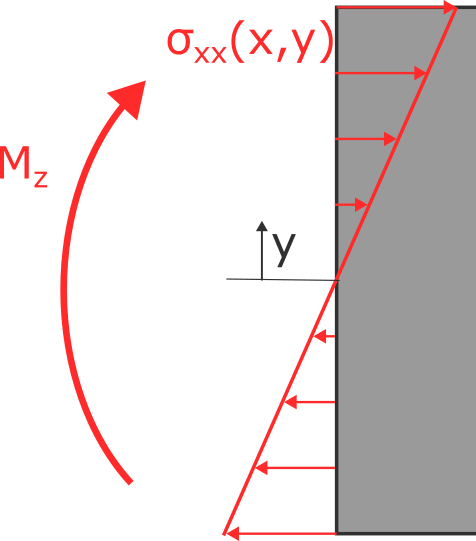
\includegraphics[scale=0.8]{Figures/5-Viga/Momento_res.png}
            \caption{Equilíbrio de forças na seção da viga}
            \label{fig:equilibrio_secao_viga}
        \end{figure}

        \begin{equation*}
            F_x = \int_A \sigma_{xx} dA = 0
        \end{equation*}

        \begin{equation*}
            F_x = -\frac{E}{\rho(x)} \int_A y dA = 0
        \end{equation*}

        \noindent a integral de área é pela área da seção transversal, que é função de $y$ e $z$, portanto, o termo $\rho(x)$ é constante e pode ser movido para fora.

        A expressão $\int_A y dA$ é o primeiro momento de área. Ela pode ser usada para encontrar a posição da linha neutra na estrutura. O resultado obtido aqui indica que a linha neutra deve passar pelo centroide da seção transversal.

        Da mesma forma, o momento resultante deve ser igual ao momento fletor (se atente aos sinais da expressão, conforme a regra da mão direita):

        \begin{equation*}
            -M_z - \int_A y \sigma_{xx} dA = 0
        \end{equation*}

        \begin{equation*}
            M_z = \frac{E}{\rho(x)} \int_A y^2 dA = \frac{EI_{zz}}{\rho}
        \end{equation*}

        \noindent no qual $I_{zz}$ será o momento de inércia da seção transversal em relação ao eixo z que passa pelo seu centroide.

        \begin{equation}
            \frac{1}{\rho} = \frac{M_z}{EI_{zz}}
        \end{equation}

        \begin{equation}
            \sigma_{xx}(x,y) = -\frac{M_z}{I_{zz}}y
        \end{equation}

        A tensão, na viga, portanto, deve ser máxima nas extremidades da seção transversal e onde se encontram os maiores valores de momento fletor.

        Finalmente, precisamos correlacionar as deflexões e o ângulo de inclinação com o raio de curvatura. Para isso, considere novamente a viga da Figura \ref{fig:deslocamento_viga}. Considerando pequenas deformações e deslocamentos, com ângulos pequenos de inclinação:

        \begin{equation}
            \frac{dv}{dx} = \theta(x)
            \label{eq:viga_defl}
        \end{equation}

        \begin{equation}
            \frac{d\theta}{dx} = \frac{1}{\rho}
            \label{eq:viga_angulo}
        \end{equation}


        Finalmente, juntando Eq. \eqref{eq:viga_equilibrio}, a Eq. \eqref{eq:viga_angulo} e Eq. \eqref{eq:viga_defl}:

        \begin{equation}
            \frac{d^2}{dx^2}\left(EI_{zz}\frac{d^2v}{dx^2}\right) = q(x)
        \end{equation}

        Considerando que a viga tem seção transversal constante e material uniforme:

        \begin{equation}
            EI_{zz}\frac{d^4v}{dx^4} = q(x)
        \end{equation}

        Para obtermos as outras grandezas, podemos integrar sucessivamente:

        \begin{equation}
            \theta(x) = \frac{dv}{dx}
        \end{equation}

        \begin{equation}
            M_z(x) = EI_{zz}\frac{d\theta}{dx} = EI_{zz}\frac{d^2v}{dx^2}
        \end{equation}

        \begin{equation}
            V_y(x) = \frac{dM_z}{dx} = EI_{zz}\frac{d^2\theta}{dx^2} = EI_{zz}\frac{d^3v}{dx^3}
        \end{equation}


    \subsection{Funções de sigularidade}

        Para resolver esta equação diferencial, usamos novamente as funções de singularidade. Neste caso, no entanto, usamos também a função $\left\langle x-a\right\rangle^{-2}$, a derivada do delta de Dirac. Esta é utilizada para representar binários aplicados na viga. A Figura \ref{fig:singularidade_viga} mostra algumas funções de singularidade, incluindo esta.

        \begin{figure}[h!]
            \centering
            
\includegraphics[scale=1.4]{Figures/5-Viga/Singularidade.pdf}
            \caption{Funções de singularidade usadas para a solução da equação da viga}
            \label{fig:singularidade_viga}
        \end{figure}

        A próxima seção mostrará alguns exemplos de solução de vigas usando essas funções.

    \subsection{Exemplo}

        Encontre o deslocamento, rotação, momento fletor e esforço cortante da viga da Figura \ref{fig:viga_exemplo_analit} usando funções de singularidade. Considere $EI_{zz} = 10^3$ Nm$^2$.

        \begin{figure}[h!]
            \centering
            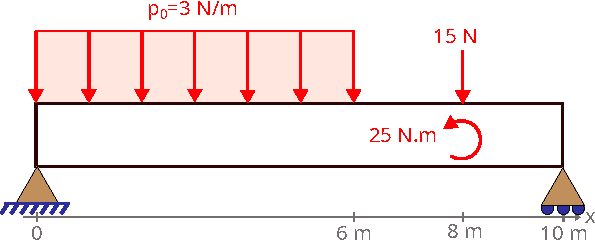
\includegraphics[scale=1]{Figures/5-Viga/Exemplo.pdf}
            \caption{Viga a ser resolvida no exemplo}
            \label{fig:viga_exemplo_analit}
        \end{figure}

        \subsubsection*{Solução}

        A força pode ser escrita como:

        \begin{equation*}
            q(x) = -3 + 3\sing{x}{6}{0} - 15\sing{x}{8}{-1} - 25\sing{x}{8}{-2}
        \end{equation*}


        As condições de contorno são: deslocamento fixo em ambas as extremidades $v(0) = v(10) = 0$ e rotação livre nas extremidades $M_z(0) = M_z(10) = 0$. Portanto:

        \begin{equation*}
            \left\{
            \begin{array}{l}
                EI_{zz}\frac{d^4v}{dx^4} = -3 + 3\sing{x}{6}{0} - 15\sing{x}{8}{-1} - 25\sing{x}{8}{-2}\\
                v(0) = 0\\
                v(10) = 0\\
                M_z(0) = EI_{zz}v''(0) = 0\\
                M_z(10) = EI_{zz}v''(10) = 0
            \end{array}
            \right.
        \end{equation*}

        Para resolver, integramos sucessivamente:

        \begin{equation*}
            V_y(x) = EI_{zz}v'''(x) = -3x + 3\sing{x}{6}{1} - 15\sing{x}{8}{0} - 25\sing{x}{8}{-1} + C_1
        \end{equation*}

        \begin{equation*}
            M_z(x) = EI_{zz}v''(x) = -\frac{3}{2}x^2 + \frac{3}{2}\sing{x}{6}{2} - 15\sing{x}{8}{1} - 25\sing{x}{8}{0} + C_1 x + C_2
        \end{equation*}

        Já podemos aplicar duas condições de contorno:

        \begin{equation*}
            M_z(0) = 0 \rightarrow C_2 = 0
        \end{equation*}

        \begin{equation*}
            M_z(10) = 0 \rightarrow -\frac{3}{2}10^2 + \frac{3}{2}\sing{10}{6}{2} - 15\sing{10}{8}{1} - 25\sing{10}{8}{0} + 10 C_1 = 0
        \end{equation*}

        \begin{equation*}
            C_1 = 18.1 Nm
        \end{equation*}

        Portanto:

        \begin{equation*}
            M_z(x) = EI_{zz}v''(x) = -\frac{3}{2}x^2 + \frac{3}{2}\sing{x}{6}{2} - 15\sing{x}{8}{1} - 25\sing{x}{8}{0} + 18.1 x
        \end{equation*}

        Continuando a integração:

        \begin{equation*}
            EI_{zz}v'(x) = EI_{zz}\theta(x)= -\frac{1}{2}x^3 + \frac{1}{2}\sing{x}{6}{3} - \frac{15}{2}\sing{x}{8}{2} - 25\sing{x}{8}{1} + \frac{18.1}{2} x^2 + C_3
        \end{equation*}

        \begin{equation*}
            EI_{zz}v(x) = -\frac{1}{8}x^4 + \frac{1}{8}\sing{x}{6}{4} - \frac{5}{2}\sing{x}{8}{3} - \frac{25}{2}\sing{x}{8}{2} + \frac{18.1}{6} x^3 + C_3 x + C_4
        \end{equation*}

        Aplicando as outras duas condições de contorno:

        \begin{equation*}
            v(0) = 0 \rightarrow C_4 = 0
        \end{equation*}

        \begin{equation*}
            v(10) = 0 \rightarrow -\frac{1}{8}10^4 + \frac{1}{8}\sing{10}{6}{4} - \frac{5}{2}\sing{10}{8}{3} - \frac{25}{2}\sing{10}{8}{2} + \frac{18.1}{6} 10^3 + 10C_3 = 0
        \end{equation*}

        \begin{equation*}
            C_3 = -17.387 Nm
        \end{equation*}

        O deslocamento, portanto, é:

        \begin{equation*}
            v(x) = \frac{1}{EI_{zz}}\left[-\frac{1}{8}x^4 + \frac{1}{8}\sing{x}{6}{4} - \frac{5}{2}\sing{x}{8}{3} - \frac{25}{2}\sing{x}{8}{2} + \frac{18.1}{6} x^3 - 17.387 x \right] [m]
        \end{equation*}

        \begin{equation*}
            v(x) = -\frac{1}{8}x^4 + \frac{1}{8}\sing{x}{6}{4} - \frac{5}{2}\sing{x}{8}{3} - \frac{25}{2}\sing{x}{8}{2} + \frac{18.1}{6} x^3 - 17.387 x [mm]
        \end{equation*}


        Integrando sucessivamente para voltar às outras grandezas:

        \begin{equation*}
            \theta(x) = \frac{1}{10^3}\left[-\frac{1}{2}x^3 + \frac{1}{2}\sing{x}{6}{3} - \frac{15}{2}\sing{x}{8}{2} - 25\sing{x}{8}{1} + \frac{18.1}{2} x^2 - 17.387\right] [rad]
        \end{equation*}

        \begin{equation*}
            M_z(x) = -\frac{3}{2}x^2 + \frac{3}{2}\sing{x}{6}{2} - 15\sing{x}{8}{1} - 25\sing{x}{8}{0} + 18.1 x [Nm]
        \end{equation*}

        \begin{equation*}
            V_y(x) = -3x + 3\sing{x}{6}{1} - 15\sing{x}{8}{0} + 18.1 [N]
        \end{equation*}

        \noindent note que as funções de singularidade com expoente menor que zero somem das expressões (visto que são funções nulas em qualquer ponto, exceto na singularidade).

        As funções acima são plotadas na Figura \ref{fig:viga_ex_curvas}.

        \begin{figure}
            \begin{subfigure}{0.99\textwidth}
                \centering
                
\includegraphics[scale=0.7]{Figures/5-Viga/deslocamento_ex1.png}
                \caption{}
            \end{subfigure}\\
            \begin{subfigure}{0.99\textwidth}
                \centering
                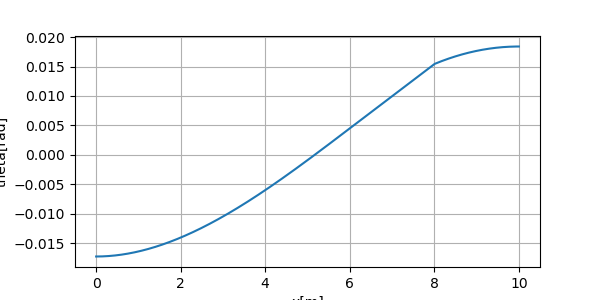
\includegraphics[scale=0.7]{Figures/5-Viga/angulo_ex1.png}
                \caption{}
            \end{subfigure}\\
            \begin{subfigure}{0.99\textwidth}
                \centering
                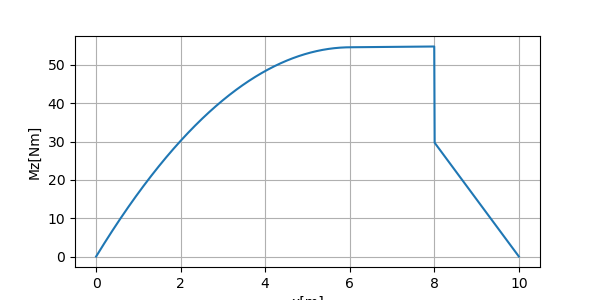
\includegraphics[scale=0.7]{Figures/5-Viga/fletor_ex1.png}
                \caption{}
            \end{subfigure}\\
            \begin{subfigure}{0.99\textwidth}
                \centering
                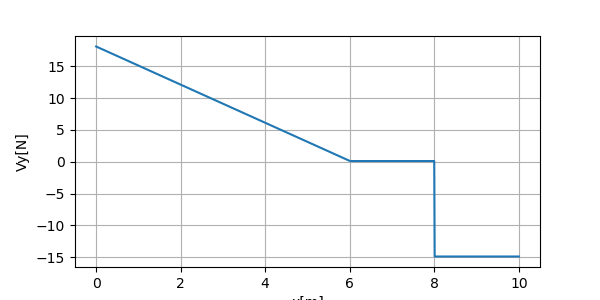
\includegraphics[scale=0.7]{Figures/5-Viga/cortante_ex1.png}
                \caption{}
            \end{subfigure}\\
            \caption{Curvas da viga do Exemplo. (a) Deflexão, (b) rotação, (c) momento fletor e (d) esforço cortante.}
            \label{fig:viga_ex_curvas}
        \end{figure}

